\documentclass{article}
\usepackage[utf8]{inputenc}
\usepackage[english]{babel}
\usepackage{graphicx}
\usepackage{geometry}
\usepackage{float}
\geometry{
	left=1in,
	right=1in,
	top=.2in,
	bottom=.2in,
}

\usepackage{multicol}
\setlength{\columnsep}{1cm}

\title{\fontfamily{phv}\textbf{Exploration of Possible Render Techniques using Pixel Shader Ordering}}
\author{Bryan Pawlowski \\ \textit{Oregon State University}}
\date{}

\begin{document}

\maketitle

\begin{figure}[H]
	\centering
	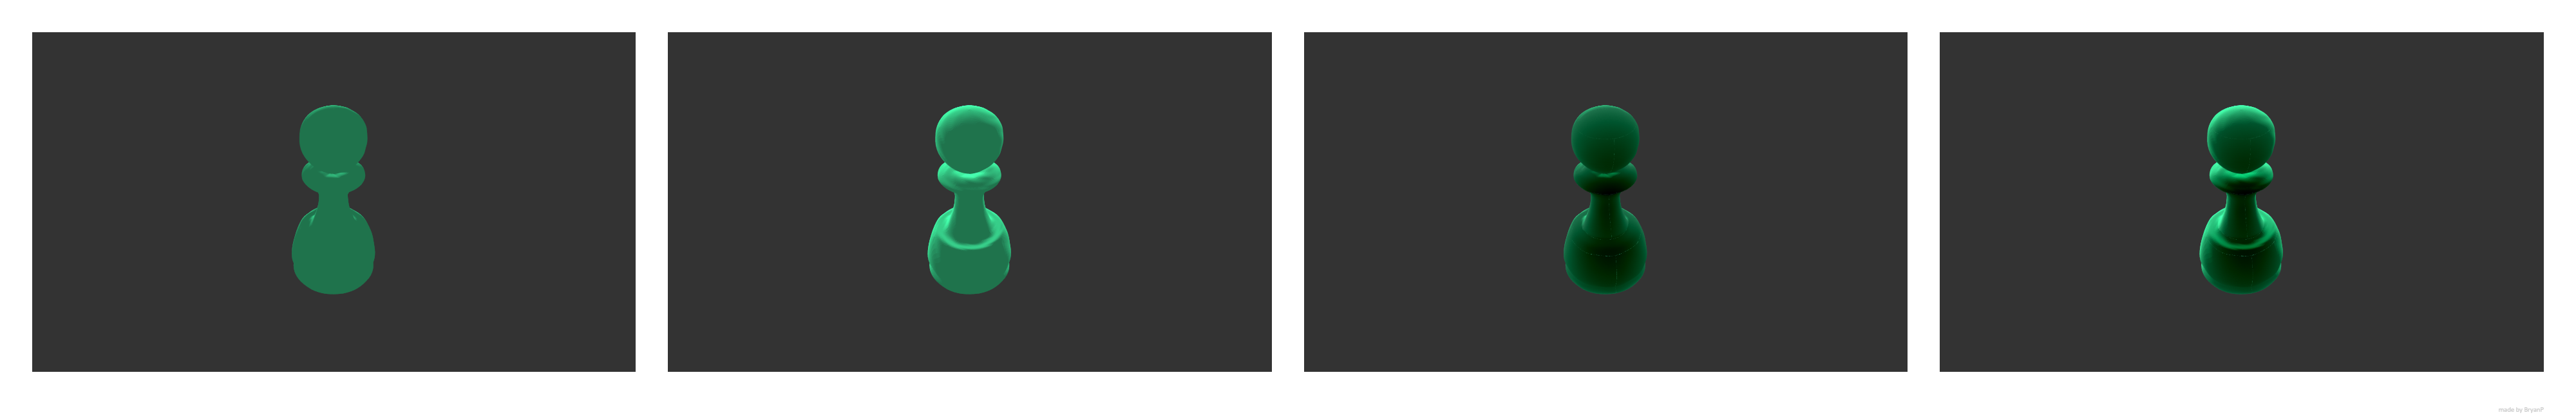
\includegraphics[width=1.0\textwidth]{ResultPicture.png}
	\caption{\textit{From left to right, Phong Smooth Shading, Phong with Normal Wrapping, Phong with Iris\texttrademark-powered depth map, then Phong with a combination of Smooth Shading and Iris\texttrademark-powered Depth Map.}}
	\label{fig: ResultPhotos}
\end{figure}

\begin{multicols*}{2}  

\section*{\fontfamily{phv}\textbf{Introduction}}

In the early stages of graphics programming, we, the programmers had a very
basic job to do in the eyes of the GPU. We were to give the GPU information on
the 3D object, set various contexts and modes, then we told the GPU to draw.
Once these fixed-function GPUs began the draw, our influence on them stopped
there. Years later, we were given the ability to actually program the GPU's
pipeline stages, first starting with a programmable vertex and fragment/pixel
shader, then getting increasingly complex. The advent of programmable shaders
gave graphics programmers the chance to unlock the GPU's potential to render a
large number of what the programmer could think of. However, there remained
the issue that we couldn't program the GPU to set barriers. Since the main
draw of a GPU is nice images quickly, it would make sense why synchronization
was never really factored into a Graphics Processor's architecture. Recently,
this has changed.
\\ \\
With the advent of Iris\texttrademark Pro, programmers are given the ability
to put a barrier and order the potential pixels being processed. This
functionality is called \textbf{Pixel Ordering} or \textbf{Pixel
Synchronization}. Given this new capability, programmers are now able to build
knowledge of entire objects in a single pass, when coupled with the use of
\textbf{Unordered Access Views} (\textbf{UAVs}). UAVs are a data structure
that allow for shared memory access between pixel shaders, and are commonly
used in compute shaders. One problem with using UAVs within a pixel shader is
that, per pixel, a programmer had no way of guaranteeing access to the UAVs.
now, with the addition of Pixel Synchronization, we are now able to guarantee
that parts of the UAV will be accessed in a deterministic order. When pixel
ordering is invoked within the pixel shader, a barrier based on screen space
is created. What this means is that each pixel in flight at the same (X, Y)
screen position hits this barrier, is ordered based upon primitive, then each
pixel in flight at that (X,Y) screen position executes one-at-a-time.

\section*{\fontfamily{phv}\textbf{My Work}}

THe main purpose of my work is to answer the question of whether or not the
Pixel Synchronization hardware capability can be used for more than the
examples that intel has set forth, and whether it is able to be efficiently
utilized to help enhance existing render techniques.

\subsubsection*{\fontfamily{phv}\textbf{Subsurface Scattering Approximation}}

Using a two-pass method, we can find a depth map of the object with respect to
the light source. Using this depth info, on the third and final pass of this
rendering technique, we modify the diffuse color based on the depth of the
model with respect to the light. I compare a few differenct characteristics of
the performance of different algorithms, including regular phong smoothing,
diffuse wrapping(as detailed by the nVidia book. Find this info), the Pixel
Ordering Subsurface scattering approximation, a combination of the diffuse
wrapping and the Pixel Ordering technique, and a smarter utilization of the
Pixel Ordering technique.

\subsubsection*{\fontfamily{phv}\textbf{Accurate Complex Model Refraction}}

In this demonstration, I will use pixel ordering to create a voxelization of
the model, then trace through the interior of the model based on the vector
returned from the \textit{refract} intrinsic function. Being able to traverse
through to the other side of a model will give a more accurate refraction
effect than just using the front side of the model. Again, a characterization
will be made between the normal refraction approach and the one with improved
quality using pixel synchronization.



\end{multicols*}

\end{document}
